\documentclass[12pt,a4paper]{article}

% ==========================================
% PACKAGES & CONFIGURATION
% ==========================================
\usepackage[utf8]{inputenc}
\usepackage[margin=1in]{geometry}
\usepackage{amsmath,amssymb,amsfonts}
\usepackage{graphicx}
\usepackage{booktabs}
\usepackage{tabularx}
\usepackage{enumitem}
\usepackage{hyperref}
\usepackage{xcolor}
\usepackage{listings}
\usepackage{tcolorbox}
\usepackage{titlesec}
\usepackage{tikz}
\usetikzlibrary{shapes.geometric, arrows.meta, positioning, fit, backgrounds, calc}
\usepackage{algorithm}
\usepackage{algpseudocode}

% --- Hyperref Setup ---
\hypersetup{
    colorlinks=true,
    linkcolor=blue!70!black,
    citecolor=blue!70!black,
    urlcolor=blue!70!black
}

% --- Code Listing Setup ---
\definecolor{codegray}{rgb}{0.5,0.5,0.5}
\definecolor{codebg}{rgb}{0.97,0.97,0.98}
\definecolor{codegreen}{rgb}{0.13,0.54,0.13}
\lstdefinestyle{mystyle}{
    backgroundcolor=\color{codebg},
    commentstyle=\color{codegreen},
    keywordstyle=\color{blue!80!black}\bfseries,
    numberstyle=\tiny\color{codegray},
    stringstyle=\color{red!70!black},
    basicstyle=\ttfamily\footnotesize,
    breakatwhitespace=false,
    breaklines=true,
    captionpos=b,
    keepspaces=true,
    numbers=left,
    numbersep=5pt,
    showspaces=false,
    showstringspaces=false,
    showtabs=false,
    tabsize=2,
    frame=single,
    rulecolor=\color{black!20}
}
\lstset{style=mystyle}

% --- TikZ Global Styles ---
\tikzset{
    baseblock/.style={rectangle, draw=black!75, rounded corners=3pt, text centered, font=\small\sffamily, inner sep=6pt},
    agentblock/.style={baseblock, draw=blue!80!black, fill=blue!8, minimum height=2.2em, minimum width=3.6cm},
    databox/.style={baseblock, draw=teal!80!black, fill=teal!8, minimum height=2.2em, minimum width=3.4cm},
    processblock/.style={baseblock, draw=orange!80!black, fill=orange!8, minimum height=2.2em, minimum width=3.6cm},
    decision/.style={diamond, draw=red!80!black, fill=red!8, aspect=1.8, text centered, font=\footnotesize\sffamily, inner sep=3pt},
    arrow/.style={thick, ->, >=stealth, color=black!80},
    line/.style={thick, color=black!80}
}

% ==========================================
% DOCUMENT METADATA
% ==========================================
\title{\textbf{\LARGE EduTwin: Multi-Agent Orchestration, Intent Routing, and Pedagogical Diagnostics Architecture}\\[0.5em]
\large Technical Report on Agent Ecosystem Design, Structured Communication Contracts, and Behavioral Verification}
\author{\textbf{Osama} \\
\textit{AI Agents \& Orchestration Lead} \\
EduTwin Project}
\date{\today}

\begin{document}

\maketitle

\begin{abstract}
\noindent This technical report documents the complete architectural design, engineering implementation, prompt design, and behavioral verification of the AI Agent Ecosystem developed for the \textbf{EduTwin} personalized educational platform. While conventional conversational educational chatbots rely on single-prompt interactions or stateless completions, EduTwin introduces a multi-agent orchestration architecture capable of intent classification, specialized pedagogical coaching, long-term career mentoring, system-level explainability, and bidirectional diagnostic signaling with a persistent Digital Twin. 

Specifically, this report covers: (1) the central \texttt{AgentOrchestrator} and multi-turn execution pipeline; (2) the Gemini-powered \texttt{IntentClassifier} equipped with structured output schemas and heuristic failovers; (3) Pydantic V2 structured data contracts and validation mechanisms; (4) the pedagogical reasoning engine of the \textbf{Study Coach} agent, including prerequisite anchoring, learning-style adaptation, and six diagnostic signals; (5) the \textbf{Career Mentor} agent's skill-gap diffing and prerequisite-aware ranking algorithm; (6) the \textbf{Explainability} agent's grounded decision justification framework; (7) robust XML-tagged output parsing; and (8) comprehensive scenario-based behavioral evaluations across academic, career, and explainability domains.
\end{abstract}

\newpage
\tableofcontents
\newpage

% ==========================================
% 1. INTRODUCTION & SCOPE
% ==========================================
\section{Introduction and Scope of Responsibilities}
\label{sec:intro}

In the EduTwin architecture, the \textbf{Agent Layer} serves as the cognitive reasoning engine bridging the student's natural-language dialogue, the structured beliefs of the \textbf{Student Digital Twin}, and the system's underlying capabilities. 

\subsection{Scope of Module Responsibilities}
My core engineering and research responsibilities in the EduTwin project encompassed the entire AI agent ecosystem and orchestration pipeline (with the sole exception of the recommendation retrieval/ranking algorithm developed by the Recommendation team). Specifically, this included:
\begin{itemize}[noitemsep,topsep=2pt]
    \item \textbf{Agent Orchestrator}: Central dispatcher handling context injection, conversation history tracking, target agent execution, and signal aggregation.
    \item \textbf{Intent Classifier \& Routing}: Machine-learning and heuristic classification routing student inputs to canonical intents and target agents.
    \item \textbf{Data Schemas \& Type Contracts}: Comprehensive Pydantic models for intent decisions, diagnostic signals, career reports, and unified execution results.
    \item \textbf{Study Coach Agent}: Pedagogical AI agent designed to diagnose knowledge gaps, resolve misconceptions, adapt depth based on prerequisite mastery, and emit real-time diagnostic signals.
    \item \textbf{Career Mentor Agent}: Long-term guidance agent performing career destination modeling, prerequisite-aware skill diffing, interest-based tiebreaking, and milestone/goal-change proposal generation.
    \item \textbf{Explainability Agent}: System transparency engine providing grounded justifications for AI decisions scaled to interaction stakes.
    \item \textbf{Output Parsers}: Fault-tolerant regex and JSON extraction pipelines isolating student-facing dialogue from structured backend signals.
    \item \textbf{Behavioral Verification}: Rigorous evaluation frameworks ensuring adherence to pedagogical, career, and explainability constraints.
\end{itemize}

% ==========================================
% 2. MULTI-AGENT ORCHESTRATION ARCHITECTURE
% ==========================================
\section{Multi-Agent System Architecture}
\label{sec:architecture}

The agent layer is structured around an asynchronous, decoupled orchestration pattern. The orchestrator receives the student's query, conversational history, and a synthesized \textit{Briefing} from the Digital Twin, dispatches the request to the appropriate specialized agent, and parses the output into student-facing text and structured diagnostic metadata.

\begin{figure}[htbp]
\centering
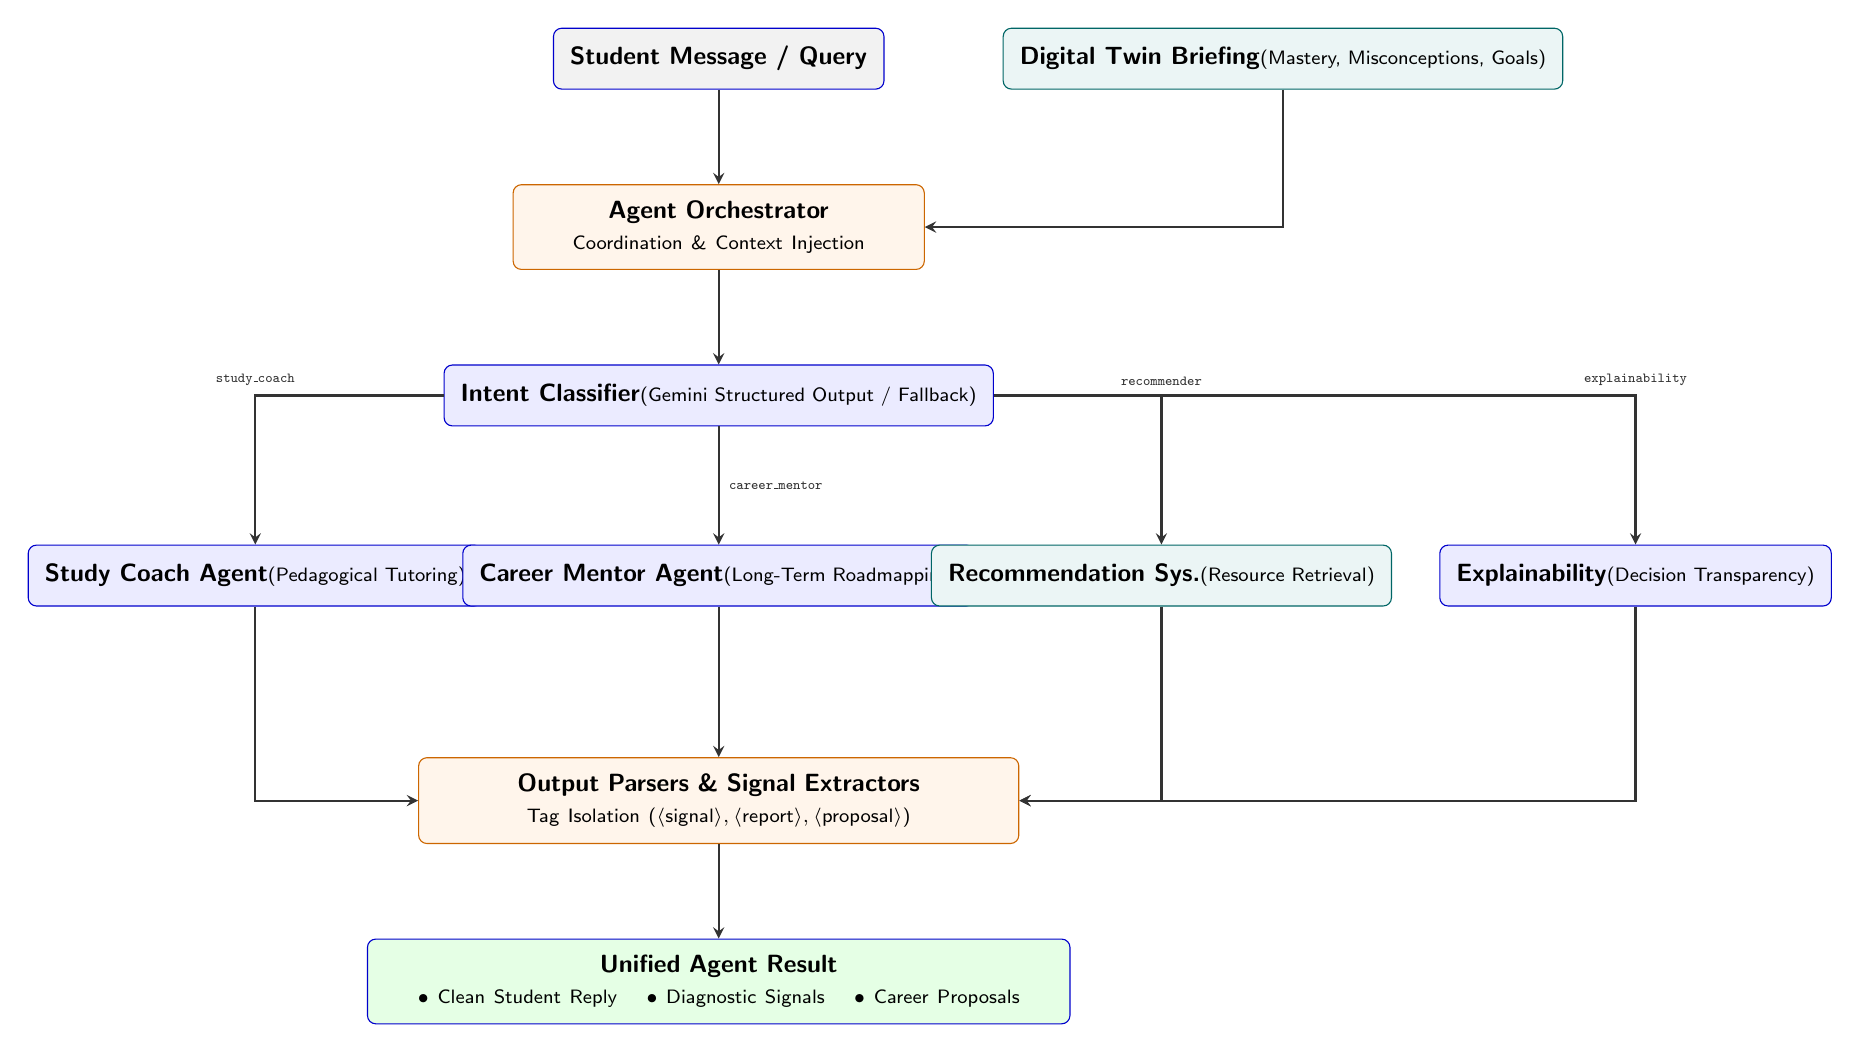
\begin{tikzpicture}[node distance=1.1cm and 1.2cm, auto]
    % Nodes
    \node (query) [agentblock, fill=gray!10] {\textbf{Student Message / Query}};
    \node (brief) [databox, right=1.5cm of query] {\textbf{Digital Twin Briefing}\\ \scriptsize (Mastery, Misconceptions, Goals)};
    
    \node (orch) [processblock, below=1.2cm of query, text width=4.8cm] {\textbf{Agent Orchestrator}\\ \scriptsize Coordination \& Context Injection};
    \node (intent) [agentblock, below=1.2cm of orch] {\textbf{Intent Classifier}\\ \scriptsize (Gemini Structured Output / Fallback)};
    
    \node (coach) [agentblock, below left=1.5cm and -0.5cm of intent] {\textbf{Study Coach Agent}\\ \scriptsize (Pedagogical Tutoring)};
    \node (mentor) [agentblock, below=1.5cm of intent] {\textbf{Career Mentor Agent}\\ \scriptsize (Long-Term Roadmapping)};
    \node (rec) [databox, below right=1.5cm and -0.8cm of intent] {\textbf{Recommendation Sys.}\\ \scriptsize (Resource Retrieval)};
    \node (exp) [agentblock, right=0.6cm of rec] {\textbf{Explainability}\\ \scriptsize (Decision Transparency)};
    
    \node (parser) [processblock, below=4.2cm of intent, text width=7.2cm] {\textbf{Output Parsers \& Signal Extractors}\\ \scriptsize Tag Isolation ($\langle\text{signal}\rangle, \langle\text{report}\rangle, \langle\text{proposal}\rangle$)};
    
    \node (result) [agentblock, below=1.2cm of parser, fill=green!10, text width=8.5cm] {\textbf{Unified Agent Result}\\ \scriptsize $\bullet$ Clean Student Reply \quad $\bullet$ Diagnostic Signals \quad $\bullet$ Career Proposals};

    % Arrows
    \draw [arrow] (query) -- (orch);
    \draw [arrow] (brief) |- (orch);
    \draw [arrow] (orch) -- (intent);
    
    \draw [arrow] (intent) -| node[above, font=\tiny] {\texttt{study\_coach}} (coach);
    \draw [arrow] (intent) -- node[right, font=\tiny] {\texttt{career\_mentor}} (mentor);
    \draw [arrow] (intent) -| node[above, font=\tiny] {\texttt{recommender}} (rec);
    \draw [arrow] (intent) -| node[above, font=\tiny] {\texttt{explainability}} (exp);
    
    \draw [arrow] (coach) |- (parser);
    \draw [arrow] (mentor) -- (parser);
    \draw [arrow] (rec) |- (parser);
    \draw [arrow] (exp) |- (parser);
    
    \draw [arrow] (parser) -- (result);
\end{tikzpicture}
\caption{End-to-End Multi-Agent Orchestration and Signal Extraction Pipeline.}
\label{fig:orchestrator_arch}
\end{figure}

\subsection{Execution Lifecycle}
The complete processing pipeline in \texttt{AgentOrchestrator} executes in four distinct phases:
\begin{enumerate}[noitemsep,topsep=2pt]
    \item \textbf{Intent Analysis}: The user query and context summary are passed to the \texttt{IntentClassifier} to yield an \texttt{IntentDecision}.
    \item \textbf{Context Formatting}: Agent-specific XML tags are assembled, including $\langle\text{conversation\_so\_far}\rangle$, $\langle\text{student\_message}\rangle$, $\langle\text{intent}\rangle$, $\langle\text{briefing}\rangle$, and (for Career Mentor) $\langle\text{role\_profile}\rangle$.
    \item \textbf{Model Invocation}: The selected agent's system instruction prompt is loaded and executed against Google Gemini with strict temperature and safety settings.
    \item \textbf{Output Separation \& Validation}: The raw text response is parsed using regular expressions to extract structured XML blocks ($\langle\text{signal}\rangle$, $\langle\text{report}\rangle$, $\langle\text{proposal}\rangle$), validate them against Pydantic models, and yield a clean text response for student rendering.
\end{enumerate}

% ==========================================
% 3. INTENT CLASSIFICATION & ROUTING
% ==========================================
\section{Intent Classification and Routing System}
\label{sec:intent}

Accurate intent routing is foundational to ensure the student interacts with a unified interface while routing execution to the optimal specialized agent.

\subsection{Canonical Intent Taxonomy}
The intent space is formally divided into four primary agent categories and eight canonical intents, as defined in Table~\ref{tab:intent_taxonomy}.

\begin{table}[htbp]
\centering
\small
\renewcommand{\arraystretch}{1.3}
\begin{tabularx}{\textwidth}{l l X}
\toprule
\textbf{Target Agent} & \textbf{Canonical Intent} & \textbf{Description \& Trigger Criteria} \\
\midrule
\texttt{study\_coach} & \texttt{explain\_concept} & Student asks for explanations of concepts, formulas, or mechanisms. \\
& \texttt{check\_answer} & Student submits reasoning or answers to verify correctness. \\
& \texttt{give\_practice} & Student requests practice problems, quizzes, or exercises. \\
\midrule
\texttt{career\_mentor} & \texttt{career\_fit\_question} & Queries regarding role requirements, industry fit, or skill needs. \\
& \texttt{progress\_alignment\_check} & Queries regarding long-term study order and milestone progress. \\
& \texttt{goal\_change} & Student declares an intention to target a new career goal. \\
\midrule
\texttt{recommendation\_system} & \texttt{resource\_recommendation} & Direct requests for external courses, books, links, or videos. \\
\midrule
\texttt{explainability} & \texttt{explain\_decision} & Inquiries into \textit{why} the system made a specific recommendation. \\
\bottomrule
\end{tabularx}
\caption{Canonical Intent Taxonomy for EduTwin Agent Routing.}
\label{tab:intent_taxonomy}
\end{table}

\subsection{Multi-Tiered Classification Strategy}
To guarantee maximum availability and prevent runtime failure, the \texttt{IntentClassifier} implements a robust 3-tier resolution strategy, illustrated in Figure~\ref{fig:intent_tiers}.

\begin{figure}[htbp]
\centering
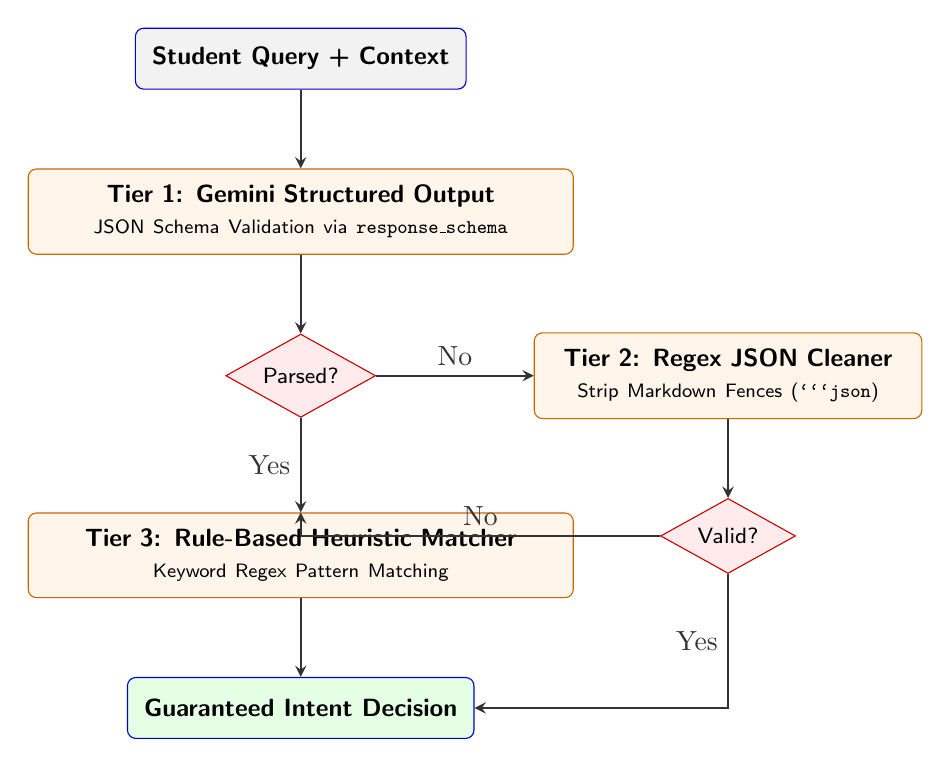
\begin{tikzpicture}[node distance=1cm, auto]
    \node (in) [agentblock, fill=gray!10] {\textbf{Student Query + Context}};
    \node (tier1) [processblock, below=of in, text width=6.5cm] {\textbf{Tier 1: Gemini Structured Output}\\ \scriptsize JSON Schema Validation via \texttt{response\_schema}};
    \node (check1) [decision, below=of tier1] {Parsed?};
    \node (tier2) [processblock, right=2cm of check1, text width=4.5cm] {\textbf{Tier 2: Regex JSON Cleaner}\\ \scriptsize Strip Markdown Fences (\texttt{```json})};
    \node (check2) [decision, below=of tier2] {Valid?};
    \node (tier3) [processblock, below=1.2cm of check1, text width=6.5cm] {\textbf{Tier 3: Rule-Based Heuristic Matcher}\\ \scriptsize Keyword Regex Pattern Matching};
    \node (out) [agentblock, below=of tier3, fill=green!10] {\textbf{Guaranteed Intent Decision}};

    \draw [arrow] (in) -- (tier1);
    \draw [arrow] (tier1) -- (check1);
    \draw [arrow] (check1) -- node[left] {Yes} (tier3);
    \draw [arrow] (check1) -- node[above] {No} (tier2);
    \draw [arrow] (tier2) -- (check2);
    \draw [arrow] (check2) |- node[near start, left] {Yes} (out);
    \draw [arrow] (check2) -| node[above, near start] {No} (tier3);
    \draw [arrow] (tier3) -- (out);
\end{tikzpicture}
\caption{Three-Tier Fault-Tolerant Intent Classification Pipeline.}
\label{fig:intent_tiers}
\end{figure}

% ==========================================
% 4. SCHEMAS & DATA CONTRACTS
% ==========================================
\section{Structured Schemas and Data Contracts}
\label{sec:schemas}

All data flowing between agents, parsers, and the Digital Twin is strictly governed by Pydantic V2 models.

\subsection{Intent Decision Schema}
The \texttt{IntentDecision} model includes custom field validators that normalize noisy LLM outputs (such as variations like \texttt{"career-mentor"}, \texttt{"tutor"}, or \texttt{"recommend"}) into typed enums:

\begin{lstlisting}[language=Python, caption={IntentDecision Schema and Normalization Logic.}]
class IntentDecision(BaseModel):
    model_config = ConfigDict(extra="ignore", populate_by_name=True)

    agent: AgentType = Field(
        default=AgentType.STUDY_COACH,
        description="The specialized agent best suited to handle the student query."
    )
    intent: str = Field(default="explain_concept")
    confidence: float = Field(default=0.0, ge=0.0, le=1.0)
    rationale: str = Field(default="")

    @field_validator("agent", mode="before")
    @classmethod
    def normalize_agent(cls, v: Any) -> AgentType:
        if isinstance(v, AgentType):
            return v
        if isinstance(v, str):
            clean = v.strip().lower().replace(" ", "_").replace("-", "_")
            for item in AgentType:
                if item.value == clean or item.name.lower() == clean:
                    return item
            # Fuzzy fallback for near-misses
            if any(k in clean for k in ["coach", "tutor", "study"]):
                return AgentType.STUDY_COACH
            if any(k in clean for k in ["career", "mentor"]):
                return AgentType.CAREER_MENTOR
            if any(k in clean for k in ["recommend", "resource"]):
                return AgentType.RECOMMENDATION_SYSTEM
            if any(k in clean for k in ["explain", "transparency"]):
                return AgentType.EXPLAINABILITY
        return AgentType.STUDY_COACH
\end{lstlisting}

\subsection{Diagnostic Signal Schema for Digital Twin Updating}
The \texttt{CoachSignal} model enables the Study Coach to communicate diagnostic findings directly to the Student Twin:

\begin{lstlisting}[language=Python, caption={CoachSignal and MentorProposal Schemas.}]
class SignalType(str, Enum):
    GAP_CONFIRMED = "gap_confirmed"
    MISCONCEPTION_DETECTED = "misconception_detected"
    MASTERY_EVIDENCE = "mastery_evidence"
    MASTERY_UNSTABLE = "mastery_unstable"
    CONFUSION_RESOLVED = "confusion_resolved"
    BRIEFING_CONTRADICTED = "briefing_contradicted"

class CoachSignal(BaseModel):
    concept: str = Field(description="Canonical concept key matching Twin ontology.")
    signal: SignalType
    detail: str = Field(description="One-sentence description of the observation.")
    evidence: str = Field(description="Direct student quote or session observation.")
    confidence: float = Field(ge=0.0, le=1.0)

class MentorProposal(BaseModel):
    type: ProposalType # goal_change_detected | milestone_completed
    detail: str
    evidence: str
    confidence: float = Field(ge=0.0, le=1.0)
\end{lstlisting}

% ==========================================
% 5. STUDY COACH AGENT
% ==========================================
\section{The Study Coach Agent}
\label{sec:coach}

The \textbf{Study Coach} is an adaptive academic tutoring agent designed to resolve a single knowledge gap or misconception per turn for a specific learner.

\subsection{Five-Step Pedagogical Reasoning Procedure}
The agent is constrained by a strict 5-step operational protocol, as depicted in Figure~\ref{fig:coach_pipeline}.

\begin{figure}[htbp]
\centering
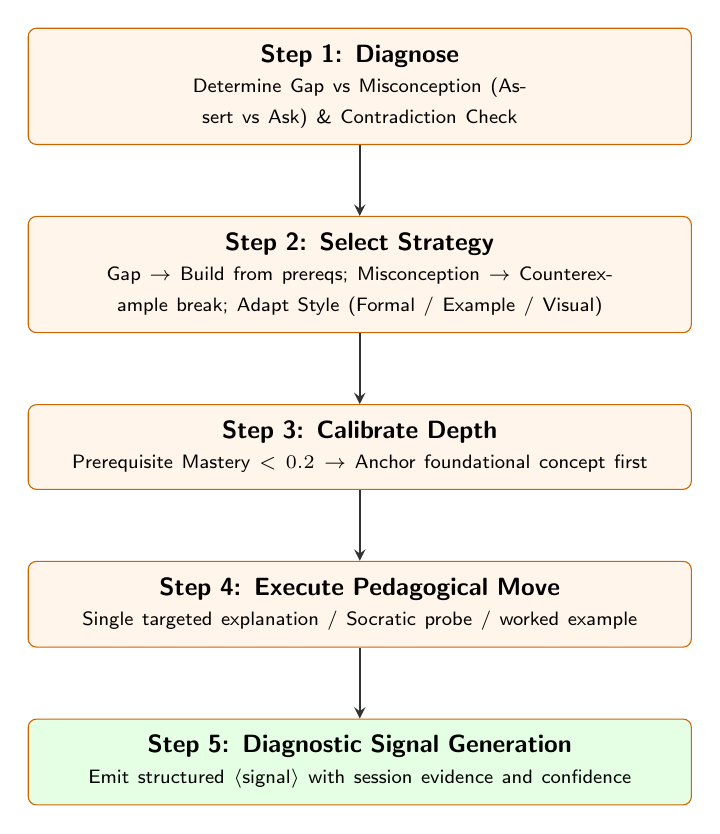
\begin{tikzpicture}[node distance=0.9cm, auto]
    \node (step1) [processblock, text width=8cm] {\textbf{Step 1: Diagnose}\\ \scriptsize Determine Gap vs Misconception (Assert vs Ask) \& Contradiction Check};
    \node (step2) [processblock, below=of step1, text width=8cm] {\textbf{Step 2: Select Strategy}\\ \scriptsize Gap $\rightarrow$ Build from prereqs; Misconception $\rightarrow$ Counterexample break; Adapt Style (Formal / Example / Visual)};
    \node (step3) [processblock, below=of step2, text width=8cm] {\textbf{Step 3: Calibrate Depth}\\ \scriptsize Prerequisite Mastery $<0.2 \rightarrow$ Anchor foundational concept first};
    \node (step4) [processblock, below=of step3, text width=8cm] {\textbf{Step 4: Execute Pedagogical Move}\\ \scriptsize Single targeted explanation / Socratic probe / worked example};
    \node (step5) [processblock, below=of step4, text width=8cm, fill=green!10] {\textbf{Step 5: Diagnostic Signal Generation}\\ \scriptsize Emit structured $\langle\text{signal}\rangle$ with session evidence and confidence};

    \draw [arrow] (step1) -- (step2);
    \draw [arrow] (step2) -- (step3);
    \draw [arrow] (step3) -- (step4);
    \draw [arrow] (step4) -- (step5);
\end{tikzpicture}
\caption{Study Coach 5-Step Pedagogical Decision Flowchart.}
\label{fig:coach_pipeline}
\end{figure}

\subsubsection{Pedagogical Decision Rules}
\begin{itemize}[noitemsep,topsep=2pt]
    \item \textbf{Assert vs. Ask Heuristic}: A student who \textit{asserts} an incorrect statement exhibits a misconception. A student who asks where something comes from or expresses confusion has a gap, even if the question contains an erroneous guess.
    \item \textbf{Contradiction Check}: If the student demonstrates correct mastery of a topic flagged as weak in the briefing (or vice versa), the agent prioritizes current session evidence over stored historical beliefs.
    \item \textbf{Learning Style Calibration}:
    \begin{itemize}[noitemsep]
        \item \textit{Formal}: Definition first, theoretical rigor, axiomatic foundations.
        \item \textit{Example-driven}: Concrete practical scenario before abstraction.
        \item \textit{Visual}: Spatial and diagrammatic analogies.
    \end{itemize}
\end{itemize}

\subsection{Diagnostic Signal Taxonomy and Semantics}
Table~\ref{tab:signals} details the semantics of all six diagnostic signals emitted by the Study Coach.

\begin{table}[htbp]
\centering
\small
\renewcommand{\arraystretch}{1.3}
\begin{tabularx}{\textwidth}{l X}
\toprule
\textbf{Signal Type} & \textbf{Trigger Condition \& Evidentiary Criteria} \\
\midrule
\texttt{gap\_confirmed} & Student confirms lack of prerequisite knowledge or asks foundational questions on an untracked/weak concept. \\
\texttt{misconception\_detected} & Student asserts a false conceptual relationship (e.g., $(f \cdot g)' = f' \cdot g'$). \\
\texttt{mastery\_evidence} & Student solves a problem or reasons correctly with high confidence. \\
\texttt{mastery\_unstable} & Student alternates between correct and incorrect answers within the same session. Replaces conflicting signals. \\
\texttt{confusion\_resolved} & Student demonstrated confusion earlier in the session but successfully proves understanding in the current turn. \\
\texttt{briefing\_contradicted} & Student's live behavior directly conflicts with stored Digital Twin briefing records. \\
\bottomrule
\end{tabularx}
\caption{Study Coach Diagnostic Signal Taxonomy.}
\label{tab:signals}
\end{table}

% ==========================================
% 6. CAREER MENTOR AGENT
% ==========================================
\section{The Career Mentor Agent}
\label{sec:mentor}

The \textbf{Career Mentor} operates at the macro-curricular level (weeks and months), aligning student progress with target professional roles.

\subsection{Role Profile Ontology \& Prerequisite Modeling}
The mentor maintains benchmark career profiles with prerequisite graphs:
\begin{equation}
    \text{Profile}(R) = \big( \{ s_i \mapsto l_i \}_{i=1}^n, \ G_{\text{prereq}} \big)
\end{equation}
where $l_i \in [0, 1]$ represents the target mastery for skill $s_i$, and $G_{\text{prereq}} = (V, E)$ is a directed acyclic graph where $(u, v) \in E$ denotes that skill $u$ is a prerequisite for skill $v$.

\begin{figure}[htbp]
\centering
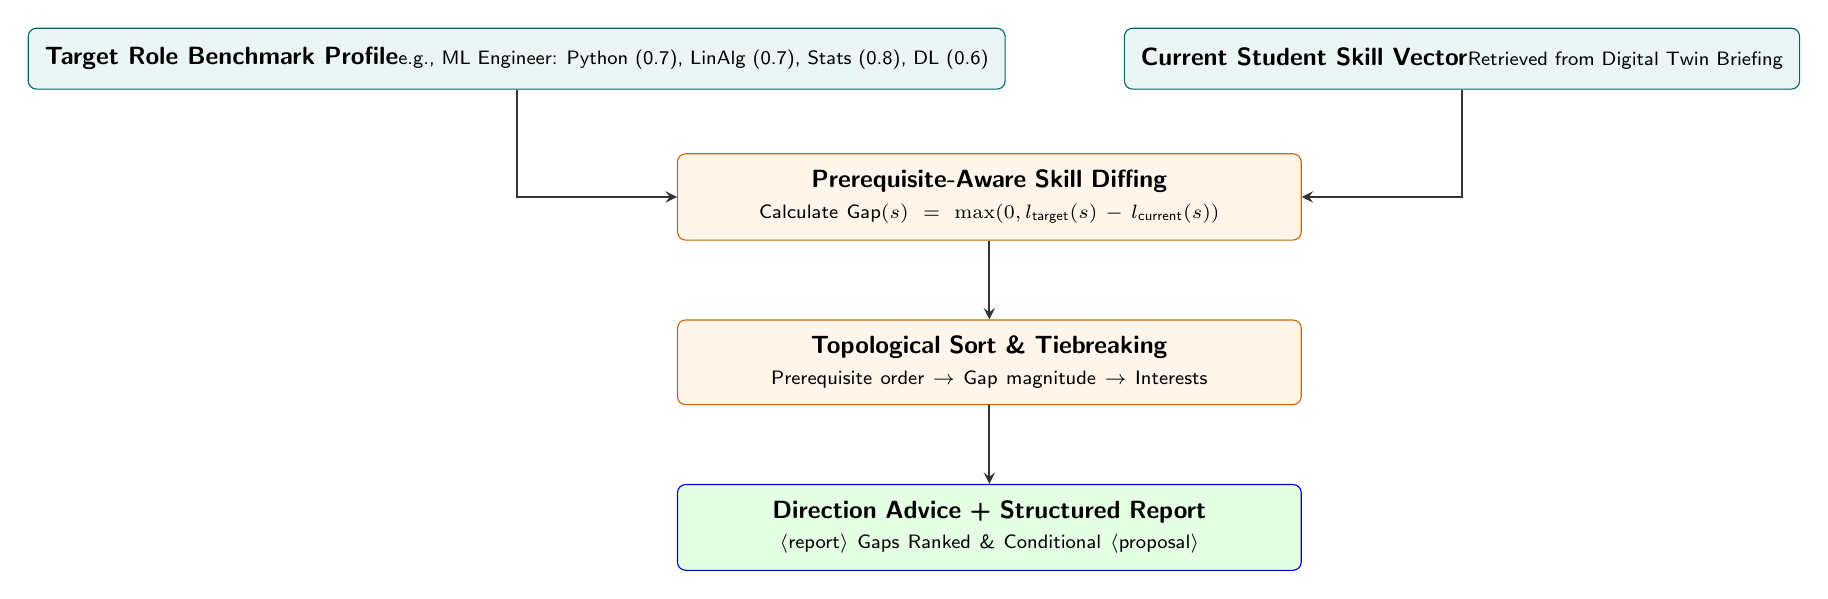
\begin{tikzpicture}[node distance=1cm, auto]
    \node (target) [databox] {\textbf{Target Role Benchmark Profile}\\ \scriptsize e.g., ML Engineer: Python (0.7), LinAlg (0.7), Stats (0.8), DL (0.6)};
    \node (current) [databox, right=1.5cm of target] {\textbf{Current Student Skill Vector}\\ \scriptsize Retrieved from Digital Twin Briefing};
    
    \node (diff) [processblock, below=1.2cm of $(target)!0.5!(current)$, text width=7.5cm] {\textbf{Prerequisite-Aware Skill Diffing}\\ \scriptsize Calculate $\text{Gap}(s) = \max(0, l_{\text{target}}(s) - l_{\text{current}}(s))$};
    
    \node (sort) [processblock, below=of diff, text width=7.5cm] {\textbf{Topological Sort \& Tiebreaking}\\ \scriptsize Prerequisite order $\rightarrow$ Gap magnitude $\rightarrow$ Interests};
    
    \node (out) [agentblock, below=of sort, fill=green!10, text width=7.5cm] {\textbf{Direction Advice + Structured Report}\\ \scriptsize $\langle\text{report}\rangle$ Gaps Ranked \& Conditional $\langle\text{proposal}\rangle$};

    \draw [arrow] (target) |- (diff);
    \draw [arrow] (current) |- (diff);
    \draw [arrow] (diff) -- (sort);
    \draw [arrow] (sort) -- (out);
\end{tikzpicture}
\caption{Career Mentor Skill Diffing and Direction Workflow.}
\label{fig:mentor_pipeline}
\end{figure}

\subsection{Prerequisite-Aware Gap Ranking Algorithm}
The mentor computes the skill gap vector:
\begin{equation}
    \text{Gap}(s_i) = \max\big(0, \ l_{\text{target}}(s_i) - l_{\text{current}}(s_i)\big)
\end{equation}
Gaps are ranked according to Algorithm~\ref{alg:mentor_ranking}.

\begin{algorithm}[htbp]
\caption{Prerequisite-Aware Career Gap Ranking}
\label{alg:mentor_ranking}
\begin{algorithmic}[1]
\Require Target Role Profile $P$, Student Skills $S_{\text{curr}}$, Student Interests $I$
\Ensure Ranked list of skill gaps $G_{\text{ranked}}$ and primary Direction $D$
\State $G \gets \emptyset$
\For{each skill $s \in P.\text{skills}$}
    \State $\delta \gets P.\text{skills}[s] - S_{\text{curr}}.get(s, 0.0)$
    \If{$\delta > 0$}
        \State $G \gets G \cup \{(s, \delta)\}$
    \EndIf
\EndFor
\State Topologically sort $G$ such that if $u \in P.\text{prerequisites}[v]$, $u$ precedes $v$.
\State For equal-depth prerequisite nodes, order by descending gap $\delta$.
\State If tied, break ties by matching with student interests $I$.
\State $G_{\text{ranked}} \gets \text{assigned priorities } 1 \dots |G|$
\State $D \gets G_{\text{ranked}}[0].\text{skill}$
\State \Return $G_{\text{ranked}}, D$
\end{algorithmic}
\end{algorithm}

\subsection{Goal Change Proposals and Frustration Filtering}
The mentor emits $\langle\text{proposal}\rangle$ objects only when explicit evidence exists. Crucially, a \textbf{Frustration Guardrail} ensures that emotional remarks (e.g., \textit{``I hate calculus, maybe I'll quit''}) are never misclassified as goal changes. Confidence scoring follows calibrated bands:
\begin{itemize}[noitemsep]
    \item $0.4 - 0.5$: Passing mention of an alternative direction.
    \item $0.6 - 0.7$: Direct statement of a new career target.
    \item $0.8 - 0.9$: Direct statement accompanied by explicit professional rationale.
\end{itemize}

% ==========================================
% 7. EXPLAINABILITY AGENT
% ==========================================
\section{The Explainability Agent}
\label{sec:explain}

The \textbf{Explainability Agent} provides transparent, verifiable justifications for recommendations or pedagogical decisions made by any module in the system.

\begin{figure}[htbp]
\centering
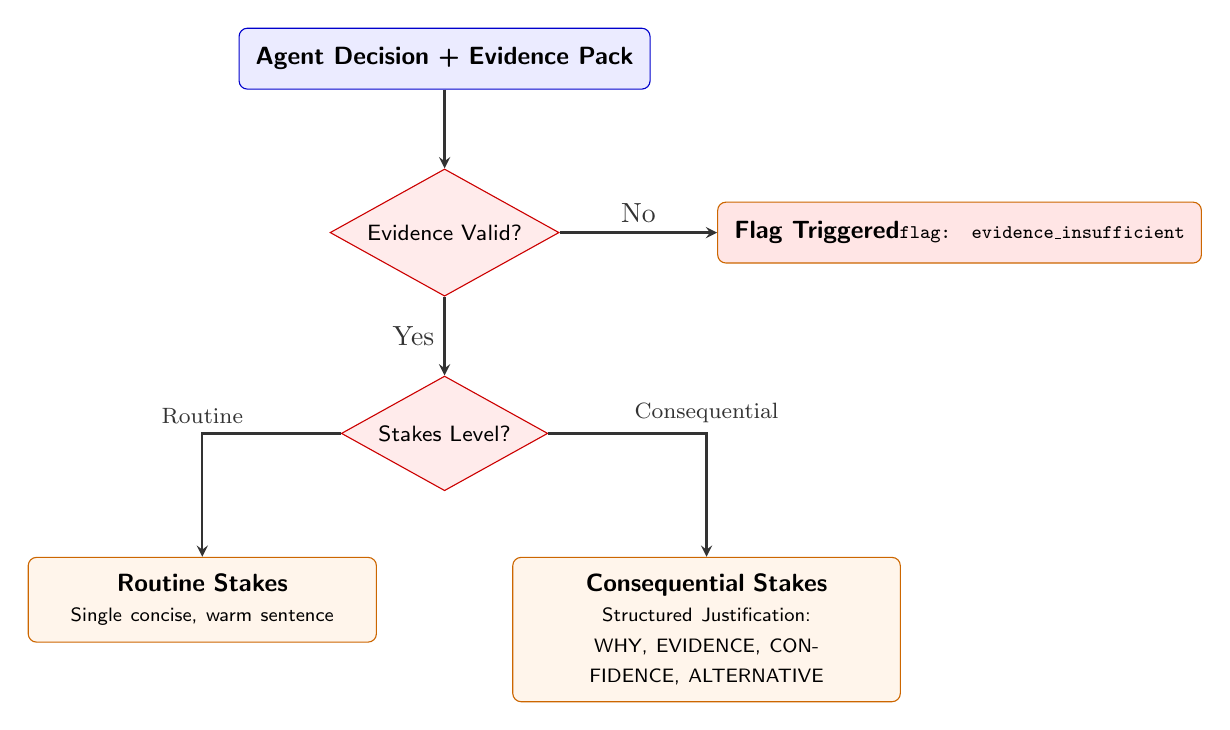
\begin{tikzpicture}[node distance=1cm, auto]
    \node (in) [agentblock] {\textbf{Agent Decision + Evidence Pack}};
    \node (check) [decision, below=of in] {Evidence Valid?};
    \node (flag) [processblock, right=2cm of check, fill=red!10] {\textbf{Flag Triggered}\\ \scriptsize \texttt{flag: evidence\_insufficient}};
    \node (stakes) [decision, below=of check] {Stakes Level?};
    
    \node (routine) [processblock, below left=1.2cm and 0.2cm of stakes, text width=4cm] {\textbf{Routine Stakes}\\ \scriptsize Single concise, warm sentence};
    \node (conseq) [processblock, below right=1.2cm and 0.2cm of stakes, text width=4.5cm] {\textbf{Consequential Stakes}\\ \scriptsize Structured Justification: WHY, EVIDENCE, CONFIDENCE, ALTERNATIVE};

    \draw [arrow] (in) -- (check);
    \draw [arrow] (check) -- node[above] {No} (flag);
    \draw [arrow] (check) -- node[left] {Yes} (stakes);
    \draw [arrow] (stakes) -| node[above, font=\footnotesize] {Routine} (routine);
    \draw [arrow] (stakes) -| node[above, font=\footnotesize] {Consequential} (conseq);
\end{tikzpicture}
\caption{Explainability Decision Justification and Stakes Scaling Pipeline.}
\label{fig:explain_pipeline}
\end{figure}

\subsection{Zero-Hallucination Grounding Rules}
The agent enforces strict evidentiary integrity constraints:
\begin{enumerate}[noitemsep,topsep=2pt]
    \item \textbf{Evidence Restriction}: Must cite \textit{only} data items present in the provided $\langle\text{evidence}\rangle$ block. Generalizing or asserting outside knowledge is prohibited.
    \item \textbf{Stakes Scaling}:
    \begin{itemize}[noitemsep]
        \item \textit{Routine}: A single, warm, concise justification sentence.
        \item \textit{Consequential}: A structured breakdown comprising \textbf{WHY}, \textbf{EVIDENCE} (2--4 bullet facts), \textbf{CONFIDENCE}, and \textbf{ALTERNATIVE} (the nearest runner-up and why it ranked lower).
    \end{itemize}
    \item \textbf{Fail-Safe Guardrail}: If the supplied evidence is insufficient to justify the decision, the agent emits the exact token \texttt{flag: evidence\_insufficient} rather than hallucinating plausible rationales.
\end{enumerate}

% ==========================================
% 8. OUTPUT PARSING
% ==========================================
\section{Response Parsing and Decoupling Engine}
\label{sec:parsers}

To maintain a clean user interface while extracting structured data for the backend, the parser module isolates XML tags using regular expressions:

\begin{figure}[htbp]
\centering
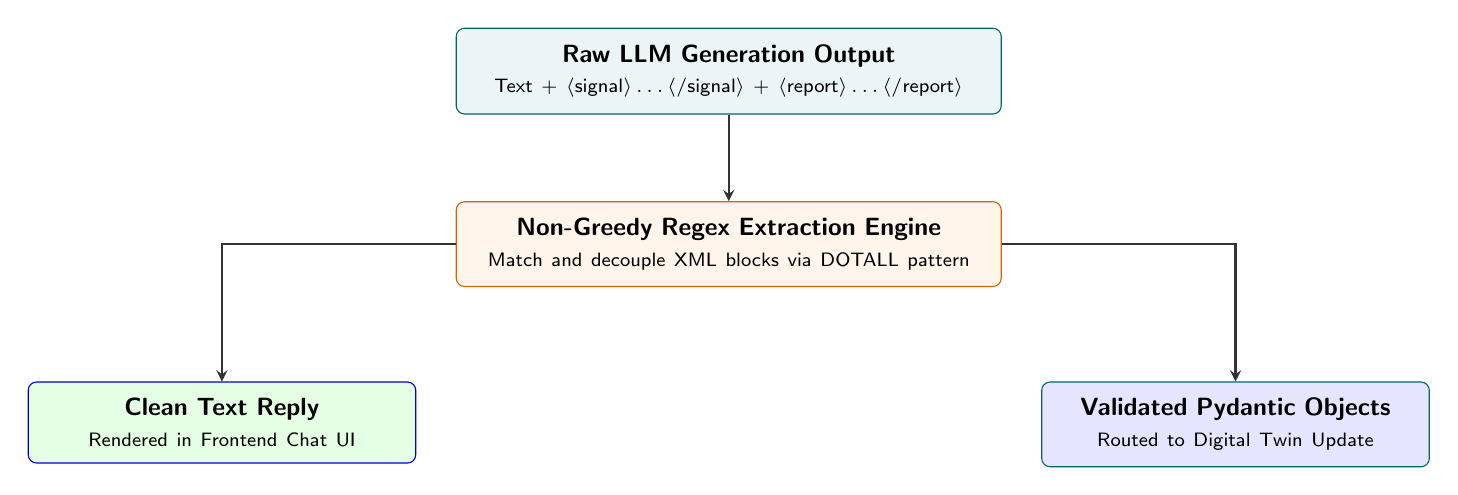
\begin{tikzpicture}[node distance=1.1cm, auto]
    \node (raw) [databox, text width=6.5cm] {\textbf{Raw LLM Generation Output}\\ \scriptsize Text + $\langle\text{signal}\rangle \dots \langle/\text{signal}\rangle$ + $\langle\text{report}\rangle \dots \langle/\text{report}\rangle$};
    
    \node (regex) [processblock, below=of raw, text width=6.5cm] {\textbf{Non-Greedy Regex Extraction Engine}\\ \scriptsize Match and decouple XML blocks via DOTALL pattern};
    
    \node (clean) [agentblock, below left=1.2cm and 0.5cm of regex, fill=green!10, text width=4.5cm] {\textbf{Clean Text Reply}\\ \scriptsize Rendered in Frontend Chat UI};
    \node (struct) [databox, below right=1.2cm and 0.5cm of regex, fill=blue!10, text width=4.5cm] {\textbf{Validated Pydantic Objects}\\ \scriptsize Routed to Digital Twin Update};

    \draw [arrow] (raw) -- (regex);
    \draw [arrow] (regex) -| (clean);
    \draw [arrow] (regex) -| (struct);
\end{tikzpicture}
\caption{Decoupling of UI Response Text and Backend Twin Signals.}
\label{fig:parser_decouple}
\end{figure}

\begin{lstlisting}[language=Python, caption={Study Coach and Career Mentor Output Parsers.}]
def parse_coach_output(raw_text: str) -> tuple[str, list[CoachSignal]]:
    signals: list[CoachSignal] = []
    raw_signals = re.findall(r"<signal>(.*?)</signal>", raw_text, re.DOTALL)
    for raw_sig in raw_signals:
        try:
            data = json.loads(raw_sig.strip())
            signals.append(CoachSignal(**data))
        except Exception:
            continue
    clean_reply = re.sub(r"<signal>.*?</signal>", "", raw_text, flags=re.DOTALL).strip()
    return clean_reply, signals

def parse_mentor_output(raw_text: str) -> tuple[str, dict[str, Any] | None, list[MentorProposal]]:
    report = None
    proposals = []
    report_match = re.search(r"<report>(.*?)</report>", raw_text, re.DOTALL)
    if report_match:
        try:
            report = json.loads(report_match.group(1).strip())
        except Exception:
            pass
    raw_props = re.findall(r"<proposal>(.*?)</proposal>", raw_text, re.DOTALL)
    for raw_p in raw_props:
        try:
            proposals.append(MentorProposal(**json.loads(raw_p.strip())))
        except Exception:
            continue
    clean_reply = re.sub(r"<report>.*?</report>", "", raw_text, flags=re.DOTALL)
    clean_reply = re.sub(r"<proposal>.*?</proposal>", "", clean_reply, flags=re.DOTALL).strip()
    return clean_reply, report, proposals
\end{lstlisting}

% ==========================================
% 9. EMPIRICAL BEHAVIORAL VERIFICATION
% ==========================================
\section{Behavioral Verification and Edge-Case Analysis}
\label{sec:eval}

The agent ecosystem was rigorously validated across 23 structural edge cases to evaluate adherence to pedagogical, roadmapping, and transparency principles.

\subsection{Study Coach Behavioral Verification}
Table~\ref{tab:coach_eval} outlines the evaluated pedagogical edge cases and verified system behaviors.

\begin{table}[htbp]
\centering
\small
\renewcommand{\arraystretch}{1.25}
\begin{tabularx}{\textwidth}{l l X c}
\toprule
\textbf{Case} & \textbf{Condition / Challenge} & \textbf{Observed \& Verified System Behavior} & \textbf{Status} \\
\midrule
\textbf{1} & Missing Concept Gap & Builds concept upward from prerequisites without assuming knowledge. & \textbf{VERIFIED} \\
\textbf{2} & Emergent Misconception & Detects false assertion, applies counterexample, and rebuilds. & \textbf{VERIFIED} \\
\textbf{3} & Formal Learning Style & Provides definition-first explanation matching formal style token. & \textbf{VERIFIED} \\
\textbf{4} & Reversing Evidence & Student initially succeeds then fails; confidence calibrated downward. & \textbf{VERIFIED} \\
\textbf{5} & Historical Contradiction & Record shows strong mastery ($0.9$), student fails; trusts live session. & \textbf{VERIFIED} \\
\textbf{6} & Prerequisite Anchoring & Prerequisite at $0.10$; anchors foundational rule before target topic. & \textbf{VERIFIED} \\
\textbf{7} & Granular Topic Matching & Matches exact sub-concept key from ontology (\texttt{chain\_rule\_inner}). & \textbf{VERIFIED} \\
\textbf{8} & Visual Learning Style & Generates spatial analogies matching visual learner profile. & \textbf{VERIFIED} \\
\textbf{9} & Confusion Resolution & Successfully emits \texttt{confusion\_resolved} after resolved struggle. & \textbf{VERIFIED} \\
\textbf{10} & Hesitation Guardrail & Hesitation leading to correct answer suppresses \texttt{mastery\_unstable}. & \textbf{VERIFIED} \\
\textbf{11} & Output Stability & Repeated evaluations show deterministic diagnostic signal generation. & \textbf{VERIFIED} \\
\bottomrule
\end{tabularx}
\caption{Study Coach Pedagogical Verification Summary.}
\label{tab:coach_eval}
\end{table}

\subsection{Career Mentor Behavioral Verification}
Table~\ref{tab:mentor_eval} details the behavioral verification of long-term career roadmapping.

\begin{table}[htbp]
\centering
\small
\renewcommand{\arraystretch}{1.25}
\begin{tabularx}{\textwidth}{l l X c}
\toprule
\textbf{Case} & \textbf{Condition / Challenge} & \textbf{Observed \& Verified System Behavior} & \textbf{Status} \\
\midrule
\textbf{1} & Prerequisite Ordering & Ranks Linear Algebra ahead of Deep Learning based on prerequisite DAG. & \textbf{VERIFIED} \\
\textbf{2} & Satisfied Skill Filtering & Omits mastered skills ($\text{gap} \le 0$) from ranked gap list. & \textbf{VERIFIED} \\
\textbf{3} & Interest Tiebreaker & Equal-gap skills broken cleanly using student declared interests. & \textbf{VERIFIED} \\
\textbf{4} & Explicit Goal Change & Stated career switch with rationale triggers proposal ($\text{conf} \ge 0.8$). & \textbf{VERIFIED} \\
\textbf{5} & Frustration Guardrail & Emotional complaint (\textit{``I hate math''}) rejects goal change proposal. & \textbf{VERIFIED} \\
\textbf{6} & Unlisted Skill Request & Refuses to invent skills missing from benchmark profile. & \textbf{VERIFIED} \\
\textbf{7} & Milestone Completion & Completed project detected and emitted as \texttt{milestone\_completed}. & \textbf{VERIFIED} \\
\textbf{8} & Unknown Target Role & Unrecognized role triggers graceful refusal without hallucination. & \textbf{VERIFIED} \\
\bottomrule
\end{tabularx}
\caption{Career Mentor Behavioral Verification Summary.}
\label{tab:mentor_eval}
\end{table}

\subsection{Explainability Grounding Verification}
Systematic verification of explainability confirmed that grounded decisions produce concise (routine) or structured (consequential) justifications, whereas ungroundable decisions reliably trigger the fail-safe \texttt{flag: evidence\_insufficient} token.

% ==========================================
% 10. CHALLENGES & FUTURE WORK
% ==========================================
\section{Engineering Challenges and Future Extensions}
\label{sec:challenges}

\subsection{Encountered Engineering Challenges}
\begin{itemize}[noitemsep,topsep=2pt]
    \item \textbf{Schema Normalization}: LLMs occasionally produce casing or naming variations in agent enums. Solved by implementing Pydantic \texttt{@field\_validator(mode="before")} with fuzzy regex mapping.
    \item \textbf{Evidentiary Leakage}: Ensuring agents cite only live session evidence rather than repeating stored briefing facts as new observations. Solved through strict prompt constraints.
    \item \textbf{XML Tag Collisions}: Prevented model markdown code blocks from corrupting XML tags by using non-greedy DOTALL regex extraction.
\end{itemize}

\subsection{Future Enhancements}
\begin{itemize}[noitemsep,topsep=2pt]
    \item \textbf{Dynamic Multi-Agent Debates}: Allowing the Study Coach and Career Mentor to debate tradeoff priorities for conflicting student goals.
    \item \textbf{Tool-Augmented Execution}: Integrating interactive Python execution sandboxes for live code and math evaluation within the Study Coach.
    \item \textbf{Streaming XML Token Parsing}: Implementing streaming SAX parsers to stream student-facing text while buffering signal XML tags concurrently.
\end{itemize}

% ==========================================
% 11. CONCLUSION
% ==========================================
\section{Conclusion}
\label{sec:conclusion}

The Agent Ecosystem designed for EduTwin establishes a robust, highly modular, and verifiable multi-agent framework. By separating pedagogical diagnosis, career roadmapping, explainability, and intent routing into specialized components governed by strict Pydantic contracts and automated diagnostic signaling, the system successfully bridges natural-language interaction with continuous Digital Twin state evolution.

Comprehensive empirical verification across 23 scenario evaluations confirms that the system reliably adheres to pedagogical constraints, handles edge cases, suppresses hallucinated goal shifts, and accurately updates student beliefs.

\end{document}
